\documentclass[aspectratio=169]{beamer}

\mode<presentation> {
	\usetheme{metropolis} 
}

\usepackage{pgfpages}

\setbeamertemplate{footline}[frame number]
\addtocounter{framenumber}{-1}

\usepackage[utf8]{inputenc}
\usepackage[czech]{babel}
\usepackage{graphicx}
\usepackage{listings}
\usepackage{fontawesome}
\usepackage{etoolbox}
\AtBeginEnvironment{frame}{\setcounter{footnote}{0}}

\title[Advanced usage of Git versioning system]{Advanced usage of Git versioning system\\ \small Git forges, automation and CI/CD}
\author{Vojtěch Trefný, Alexander Zgabur}
\date{24.~3.~2026}


\begin{document}

{\setbeamertemplate{footline}{} 
\begin{frame}
\titlepage
\end{frame}
}

\newcommand*\openquote{\makebox(25,-22){\scalebox{5}{``}}}
\newcommand*\closequote{\makebox(25,-22){\scalebox{5}{''}}}

%%%%%%%%%%%%%%%%%%%%%%%%%%%%%%%%%%%%%%%%%%%%%%%%%%%%%%%%%%%%%%%%%%

\begin{frame}
	\frametitle{Homeworks}
	
	\begin{block}{\color{orange}{Deadlines}}
		\begin{itemize}
			\item \textbf{HW 3:} 30th March 2026, 23:59
			\item \textbf{HW 4:} 13th April 2026, 23:59
		\end{itemize}
	\end{block}

	\begin{block}{\color{orange}{Homework 4}}
		\begin{itemize}
			\item Sync your fork. Open a new MR updating your \texttt{<uco>.txt} file.
			\item CI pipeline will fail on your MR.
			\item Debug the issue and update your \texttt{<uco>.txt}  to comply with new linting rules.
		\end{itemize}
	\end{block}

\end{frame}

\section{Git Forges}

\begin{frame}
	\frametitle{Git Forge}
	
	\begin{itemize}
		\item \emph{\textbf{Forge} is a web-based collaborative software platform for both developing and sharing computer applications.}\footnotemark
		\item Git forge is a forge where Git is used as the version control system.
		\item Usually offers multiple services:
		\begin{itemize}
			\item Pull/merge requests interface, including discussions and review.
			\item Issue tracker.
			\item Project management tools (e.g. Kanban board).
			\item Continuous integration (CI) and Continuous delivery (CD) tools and environment.
			\item Release management and software hosting.
			\item Wiki and/or website hosting.
		\end{itemize}
	\end{itemize}

\footnotetext[1]{\tiny\url{https://en.wikipedia.org/wiki/Forge_(software)}}

\end{frame}

\begin{frame}
	\frametitle{GitHub}
	
	\begin{columns}
		\begin{column}{0.6\textwidth}
			\begin{block}{}
				\begin{itemize}
					\item Probably the best known and most used Git forge these days. 
					\item For many, a de-facto synonym for Git.
					\item Proprietary, currently owned by Microsoft.
					\item Public projects are hosted for free, private projects are limited for non-enterprise users.
					\item Offers CI/CD integration, custom command line tool (\texttt{gh}) and integration with many third party projects.
				\end{itemize}
			\end{block}
		\end{column}
		\begin{column}{0.4\textwidth}
			\begin{figure}[ht!]
			\begin{center}
		  	  
\includegraphics[width=0.5\textwidth]{img/github-logo.png}
			\end{center}
			\end{figure}
		\end{column}
	\end{columns}

\end{frame}

\begin{frame}
	\frametitle{GitLab}
	
	\begin{columns}
		\begin{column}{0.6\textwidth}
			\begin{block}{}
				\begin{itemize}
					\item Open core Git forge used by many open source projects and organizations.
					\item Cloud-hosted \url{GitLab.com} is available for free for individuals and open source projects.
					\item Community edition (available under MIT license) can be self-hosted.
					\item Offers CI/CD integration, custom command line tool (\texttt{glab}) and integration with many third party projects.
				\end{itemize}
			\end{block}
		\end{column}
		\begin{column}{0.4\textwidth}
			\begin{figure}[ht!]
			\begin{center}
		  	  
\includegraphics[width=0.5\textwidth]{img/gitlab-logo.png}
			\end{center}
			\end{figure}
		\end{column}
	\end{columns}

\end{frame}

\begin{frame}
	\frametitle{Forgejo}

	\begin{columns}
		\begin{column}{0.6\textwidth}
			\begin{block}{}
				\begin{itemize}
					\item Open-source self-hosted Git forge.
					\item Includes integrated Wiki, Kanban board, CI (Forgejo actions), Pages, Translations etc.
					\item Projects can be migrated to Forgejo from GitHub, GitLab and others, including issues, wiki, releases etc.
					\item Public instance for hosting free and opensource projects is available on \url{Codeberg.org}.
				\end{itemize}
			\end{block}
		\end{column}
		\begin{column}{0.4\textwidth}
			\begin{figure}[ht!]
			\begin{center}
		  	  
\includegraphics[width=0.5\textwidth]{img/forgejo-logo.png}
			\end{center}
			\end{figure}
		\end{column}
	\end{columns}

\end{frame}

\section{CI/CD}

\begin{frame}
	\frametitle{What is CI/CD}

	\begin{block}{\color{orange}{Continuous Integration (CI)}}
		\begin{itemize}
			\item \emph{Practice of integrating source code changes frequently and ensuring that the integrated codebase is in a workable state.}\footnotemark
			\item Each change is automatically built and tested.
		\end{itemize}
	\end{block}

	\begin{block}{\color{orange}{Continuous Delivery / Deployment (CD)}}
		\begin{itemize}
			\item \textbf{Continuous Delivery} -- code changes are automatically prepared for release and manual deployment.
			\item \textbf{Continuous Deployment} -- every change that successfully passes the pipeline is automatically deployed to production.
		\end{itemize}
	\end{block}

\footnotetext[1]{\tiny\url{https://en.wikipedia.org/wiki/Continuous_integration}}
\end{frame}

\begin{frame}
	\frametitle{CI/CD Pipeline}

	\begin{block}{}
		\begin{itemize}
			\item Steps that need to be performed to test and deliver a new version of the software.
			\item Defines what needs to be done: when, how and in what order.
			\item Steps can vary for every project.
			\item Multiple pipelines or steps can run in parallel.
		\end{itemize}
	\end{block}
	
	\begin{figure}[ht!]
	\begin{center}
  	  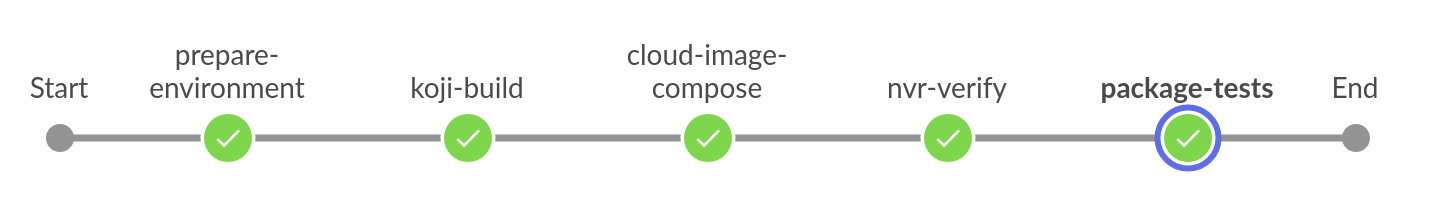
\includegraphics[width=11cm]{img/fedora-pipeline.png}
	\end{center}
	\end{figure}
\end{frame}

\begin{frame}
	\frametitle{CI/CD Pipeline}
	
\begin{columns}
\begin{column}{0.5\textwidth}
   	\begin{block}{\color{orange}{1. Testing environment}}
   		\vspace{1mm}
Preparation of the environment to run the tests: deploying containers, starting VMs...
	\end{block}
	\begin{block}{\color{orange}{2. Static Analysis}}
   		\vspace{1mm}
Finding defects by analyzing the code without running it.
     \end{block}
         \begin{block}{\color{orange}{3. Code style}}
   		\vspace{1mm}
Checking for violations of the language or project style guides.
     \end{block}
     
\end{column}
\begin{column}{0.5\textwidth}
\begin{block}{\color{orange}{4. Build}}
   		\vspace{1mm}
Building the project from source.\\~
     \end{block}
      \begin{block}{\color{orange}{5. Tests}}
   		\vspace{1mm}
Running project test suite or test suites.\\~
     \end{block}
      \begin{block}{\color{orange}{6. Packaging and Deployment}}
   		\vspace{1mm}
Building source archives, packages or container images.
     \end{block}
\end{column}
\end{columns}
\end{frame}

\begin{frame}
	\frametitle{Testing Environment}

\begin{columns}
\begin{column}{0.5\textwidth}
	\begin{figure}[ht!]
	\begin{center}
  	  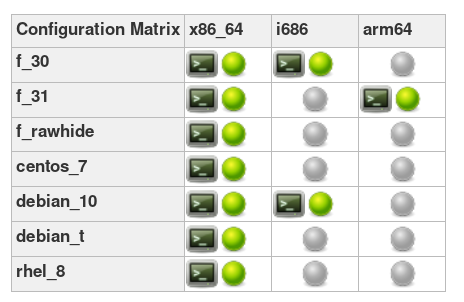
\includegraphics[width=\textwidth]{img/ci-matrix.png}
	\end{center}
	\end{figure}
\end{column}
\begin{column}{0.5\textwidth}
\begin{block}{\color{orange}{1. Preparation of VMs/containers to run the tests}}
   		\vspace{1mm}
We might want to run tests in different environments on multiple different distributions or architectures.
     \end{block}
      \begin{block}{\color{orange}{2. Installation of the test dependencies}}
   		\vspace{1mm}
Test dependencies are usually not covered by the project dependencies.
     \end{block}
      \begin{block}{\color{orange}{3. Getting the code}}
   		\vspace{1mm}
Clone the PR or get the latest code from the main branch.
     \end{block}
\end{column}
\end{columns}
\end{frame}

\begin{frame}
	\frametitle{Static Analysis}

	\begin{block}{}
		\begin{itemize}
			\item Tools that can identify potential bugs by analyzing the code without running it.
			\item Can detect problems not covered by the test suite -- corner cases, error paths etc.
				\begin{itemize}
					\item Coverity (C/C++, Java, Python, Go…)\footnotemark
					\item Cppcheck (C/C++)\footnotemark
					\item Pylint (Python)\footnotemark
					\item RuboCop (Ruby)\footnotemark
				\end{itemize}
		\end{itemize}
	\end{block}

\footnotetext[1]{\tiny\url{https://scan.coverity.com}}
\footnotetext[2]{\tiny\url{https://cppcheck.sourceforge.io/}}
\footnotetext[3]{\tiny\url{https://www.pylint.org}}
\footnotetext[4]{\tiny\url{https://docs.rubocop.org}}

\end{frame}

\begin{frame}[fragile]
	\frametitle{Coverity}
\begin{lstlisting}[frame=none, basicstyle=\ttfamily\small, escapechar=$, columns=fullflexible, keepspaces=true]
$\color{red}{Error: USE\_AFTER\_FREE (CWE-825):}$
libblockdev-2.13/src/plugins/lvm-dbus.c:1163: freed_arg: "g_free" 
frees "output".
libblockdev-2.13/src/plugins/lvm-dbus.c:1165: pass_freed_arg: Passing freed 
pointer "output" as an argument to "g_set_error".
$\color{blue}{\#}$ 1163|       g_free (output);
$\color{blue}{\#}$ 1164|       if (ret == 0) {
$\color{blue}{\#}$ 1165|->         g_set_error (error, BD_LVM_ERROR, BD_LVM_ERROR_PARSE,
$\color{blue}{\#}$ 1166|                        "Failed to parse number from output: '%s'",
$\color{blue}{\#}$ 1167|                        output);
\end{lstlisting}

\end{frame}

\begin{frame}
	\frametitle{Runtime Analysis}

	\begin{block}{}
		\begin{itemize}
			\item Tools that can identify bugs during runtime.
			\item Needs the code to actually run, either through manual testing or when running the test suite.
				\begin{itemize}
					\item Valgrind -- memory management and threading bugs\footnotemark
					\item ASan -- \emph{AddressSanitizer} -- memory management bugs (buffer overflow, dangling pointers...). Part of the LLVM project, integrated into \texttt{gcc} and \texttt{clang}\footnotemark
				\end{itemize}
		\end{itemize}
	\end{block}

\footnotetext[1]{\tiny\url{https://valgrind.org/}}
\footnotetext[2]{\tiny\url{https://github.com/google/sanitizers/wiki/AddressSanitizer}}

\end{frame}

\begin{frame}
	\frametitle{Code style and style guides}

	\begin{block}{}
		\begin{itemize}
			\item Coding conventions -- naming, code lay-out, comment style…
			\item Language specific (PEP 8\footnotemark), project specific (Linux kernel coding style\footnotemark) or library/toolkit specific (GTK coding style\footnotemark).
			\item Automatic checks using specific tools (\texttt{pycodestyle}) or (partially) by the static analysis tools.
		\end{itemize}
	\end{block}

\footnotetext[1]{\tiny\url{https://www.python.org/dev/peps/pep-0008/}}
\footnotetext[2]{\tiny\url{https://www.kernel.org/doc/html/v5.11/process/coding-style.html}}
\footnotetext[3]{\tiny\url{https://developer.gnome.org/programming-guidelines/stable/c-coding-style.html.en}}
\end{frame}

\begin{frame}
	\frametitle{Build}
	
	\begin{block}{}
		\begin{itemize}
			\item Building the project, a preparation to run the test suite.
			\item Depends on language -- mostly no-op for interpreted languages, more complicated for compiled ones.
			\item Build in the CI environment can detect issues with dependencies.
			\item Builds on different architectures can help detect issues related to endianness or data type sizes.
		\end{itemize}
	\end{block}
\end{frame}

\begin{frame}
	\frametitle{Tests}
	
	\begin{block}{}
		\begin{itemize}
			\item Running tests that are part of the project.
			\item  New tests should be part of every change to the codebase.
			\begin{itemize}
				\item New features require new unit and integration tests.
				\item Bug fixes should come with a regression test.
			\end{itemize}
			\item For some projects (like libraries) running test suites of their users might be an option.
		\end{itemize}
	\end{block}
\end{frame}

\begin{frame}
	\frametitle{Coverage}
	
	\begin{block}{}
		\begin{itemize}
			\item Code coverage (or Test coverage) represents how much of the code is covered by the test suite.
			\item Usually a percentage value that shows how many lines of the code were “visited” by the test.
			\item Generally a check that all functions and branches are covered by the suite.
			\item Used as a measure of the test suite “quality”.
		\end{itemize}
	\end{block}
\end{frame}

\begin{frame}[fragile]
	\frametitle{Coverage}
	
\begin{center}
\begin{lstlisting}[frame=none, basicstyle=\ttfamily\small, columns=fullflexible, keepspaces=true]
Name   Stmts   Miss Branch BrPart  Cover   Missing
--------------------------------------------------------------------------------
a.py     487      9    178     11    97%   206, 268, 377->376, 393->392, 418, 
                                           448, 452, 460, 660, 729, 746, 
                                           889->891, 891->894
b.py     220      8     74      8    95%   81, 173, 193->197, 279, 340, 342, 346
c.py      19      9      8      2    44%   35-36, 50->48, 53, 60-70
d.py       5      0      6      1    91%   31->exit
e.py      46      0      4      0   100%
...
--------------------------------------------------------------------------------
TOTAL   3600   1477   1381    100    56%
\end{lstlisting}
	
\end{center}
\end{frame}

\begin{frame}
	\frametitle{Packaging and publishing}
	
	\begin{block}{}
		\begin{itemize}
			\item \textbf{Delivery} -- releasing new changes quickly and regularly (daily, weekly...).
			\item \textbf{Deployment} -- delivery with automated push to production, without human interaction.
		\end{itemize}
	\end{block}
	
	\begin{block}{}
		\begin{itemize}
			\item Usually after merging the changes, not for the PRs.
			\item Building packages, container images, ISO images…
			\item Built packages can be used for further testing (manually by the Quality Assurance or in another CI infrastructure) or directly pushed to production or included in testing/nightly builds of the project.
		\end{itemize}
	\end{block}
\end{frame}

\begin{frame}
	\frametitle{Packit}

	\begin{itemize}
		\item Tool for automating packaging and testing of upstream projects for Fedora.
		\item Integrates with GitHub and GitLab: automatically builds RPM packages and runs tests on pull requests.
	\end{itemize}

	\begin{figure}[ht!]
	\begin{center}
  	  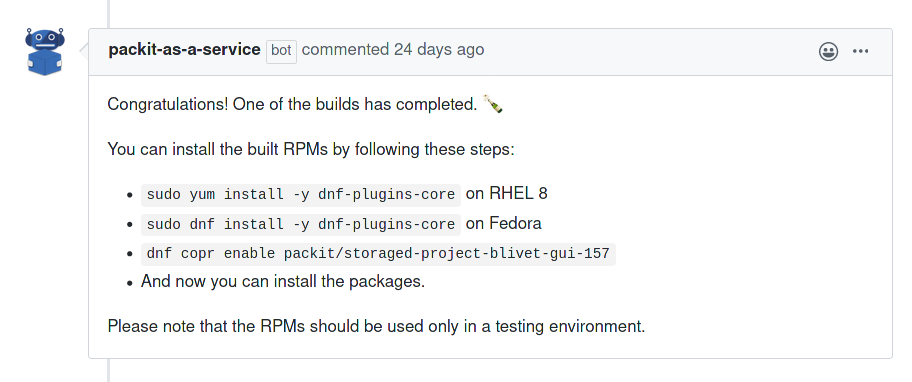
\includegraphics[width=0.8\textwidth]{img/packit-1.png}
	\end{center}
	\end{figure}
\end{frame}

%%%%%%%%%%%%%%%%%%%%%%%%%%%%%%%%%%%%%%%%%%%%%%%%%%%%%%%%%%%%%%%%%%

\section{Homework}

\begin{frame}
	\frametitle{HW 5}
	
	\begin{block}{\color{orange}{Instructions}}
		\begin{itemize}
			\item Create your own repo on GitLab (or equivalent).
			\item Set up GitLab CI or GitHub actions on the repo and create at least one action that will react to a MR/PR in some meaningful way (runs \emph{tests}, writes a comment, etc.).
			\item Open a MR/PR demonstrating the action.
			\item If you already have an existing project where this could be beneficial to you, you can use that project.
			\item \uv{Odpovědník} will be prepared where you'll fill in the URL of your repo.
		\end{itemize}
	\end{block}
	
	\begin{block}{\color{orange}{Deadline}}
		\begin{itemize}
			\item 20th April 2026, 23:59
		\end{itemize}
	\end{block}
	
\end{frame}

%%%%%%%%%%%%%%%%%%%%%%%%%%%%%%%%%%%%%%%%%%%%%%%%%%%%%%%%%%%%%%%%%%

\section{CI Tools \\ \small Demo}

\begin{frame}
	\frametitle{GitHub Actions}
	
	\begin{columns}
\begin{column}{0.6\textwidth}
	\begin{block}{}
		\begin{itemize}
			\item Automation \emph{framework} integrated into GitHub.
			\item Covers not only CI but also CD (publishing packages on various services and deploying on many public clouds) and project and issue management.
			\item Free for all public repositories, limited and paid options for private projects.
			\item \color{blue}{\url{https://github.com/features/actions}}
		\end{itemize}
	\end{block}
\end{column}
\begin{column}{0.4\textwidth}
	\begin{figure}[ht!]
	\begin{center}
  	  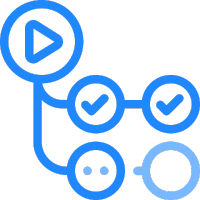
\includegraphics[width=0.5\textwidth]{img/gh-actions-logo.png}
	\end{center}
	\end{figure}
\end{column}
\end{columns}

\end{frame}

\begin{frame}[fragile]
	\frametitle{GitHub Actions -- Testing Environment Setup}
	
\begin{center}
\begin{lstlisting}[frame=none, basicstyle=\ttfamily\small, escapechar=$,columns=fullflexible, keepspaces=true]
    runs-on: ubuntu-latest			$\color{red}{<-- System to run the tests on}$

    steps:
    - uses: actions/checkout@v4			$\color{red}{<-- Getting the code}$
    - name: Set up Python 3.10
      uses: actions/setup-python@v3		$\color{red}{<-- Environment configuration}$
      with:
        python-version: "3.10"
    - name: Install dependencies
      run: |					$\color{red}{<-- Dependencies installation}$
        python -m pip install --upgrade pip
        pip install flake8 pytest
        if [ -f requirements.txt ]; then pip install -r requirements.txt; fi
\end{lstlisting}
\end{center}
\end{frame}

\begin{frame}[fragile]
	\frametitle{GitHub Actions -- Static Analysis and Tests}
	
\begin{center}
\begin{lstlisting}[frame=none, basicstyle=\ttfamily\small, escapechar=$,columns=fullflexible, keepspaces=true]
    steps:
...
    - name: Lint with flake8		$\color{red}{<-- Static analysis}$
      run: |
        # stop the build if there are Python syntax errors or undefined names
        flake8 . --count --select=E9,F63,F7,F82 --show-source --statistics
        # exit-zero treats all errors as warnings
        flake8 . --count --exit-zero --max-complexity=10 --max-line-length=127
    - name: Test with pytest		$\color{red}{<-- Tests}$
      run: |
        pytest
\end{lstlisting}
\end{center}
\end{frame}

\begin{frame}
	\frametitle{GitHub Actions Demo}
	\begin{center}
		Repository with examples used during the demo:

		\color{orange}{\large \url{https://github.com/vojtechtrefny/github-actions-examples}}
	\end{center}
\end{frame}

\begin{frame}
	\frametitle{GitLab CI}
	
	\begin{columns}
\begin{column}{0.6\textwidth}
	\begin{block}{}
		\begin{itemize}
			\item CI/CD automation integrated into GitLab.
			\item Configuration is done with a YAML file in the repository.
			\item Pipelines/tests can run either on infrastructure provided by GitLab or on custom runners.
			\item \color{blue}{\url{https://docs.gitlab.com/ee/ci/}}
		\end{itemize}
	\end{block}
\end{column}
\begin{column}{0.4\textwidth}
	\begin{figure}[ht!]
	\begin{center}
  	  
\includegraphics[width=0.5\textwidth]{img/gitlab-logo.png}
	\end{center}
	\end{figure}
\end{column}
\end{columns}

\end{frame}

\begin{frame}
	\frametitle{GitLab CI}
	\begin{figure}[ht!]
	\begin{center}
  	  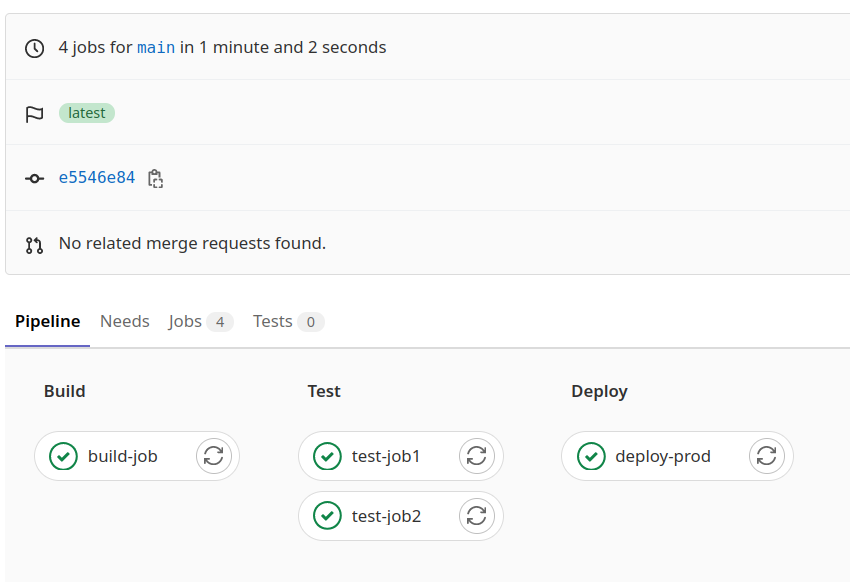
\includegraphics[width=0.8\textwidth]{img/gitlab-ci-1.png}
	\end{center}
	\end{figure}
\end{frame}

\begin{frame}
	\frametitle{GitLab CI Demo}
	\begin{center}
		Repository with examples used during the demo:

		\color{orange}{\large \url{https://gitlab.fi.muni.cz/xzgabur/github-actions-examples}}
	\end{center}
\end{frame}

\begin{frame}[fragile]
	\frametitle{GitLab CI @ FI MUNI}

	\begin{block}{\color{orange}{Continuous Integration @ GitLab FI}}
		\begin{itemize}
			\item  In \emph{Settings → General → Permissions}, enable the \emph{Pipelines} option if it is not already enabled.
			\item In the \texttt{.gitlab-ci.yml} settings, add the \texttt{.shared-fi} tag to each target, e.g.:
\begin{lstlisting}[frame=single, basicstyle=\ttfamily\small, escapechar=$,columns=fullflexible, keepspaces=true]
  build:
    tags:
      - shared-fi\end{lstlisting}
			\item More information about GitLab CI @ FI MUNI is available at
				\color{orange}{\url{https://www.fi.muni.cz/tech/unix/gitlab/ci.html}}
		\end{itemize}
	\end{block}

\end{frame}

\begin{frame}
	\frametitle{Jenkins}
	
	\begin{columns}
\begin{column}{0.6\textwidth}
	\begin{block}{}
		\begin{itemize}
			\item Automation system, not a “true” CI/CD tool.
			\item Can automatically run given tasks on a node or set of nodes.
			\item Tasks can be started on a time basis or triggered by an external event (like a new commit or PR on GitHub).
			\item \color{blue}{\url{https://jenkins.io/}}
		\end{itemize}
	\end{block}
\end{column}
\begin{column}{0.4\textwidth}
	\begin{figure}[ht!]
	\begin{center}
  	  
\includegraphics[width=0.5\textwidth]{img/jenkins.png}
	\end{center}
	\end{figure}
\end{column}
\end{columns}
\end{frame}

\end{document}

